\subsection{Database Specifications}
\subsubsection{Users and Groups}
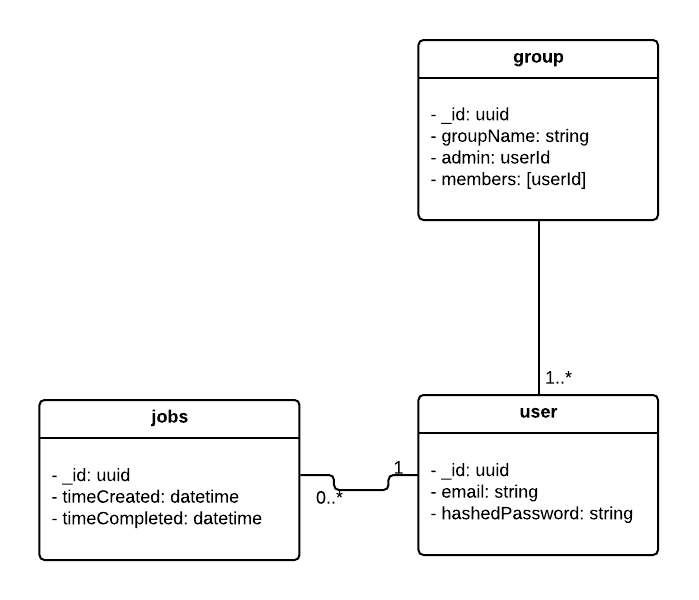
\includegraphics[width=\textwidth]{DBUML2}
A user signs up for our service using their email address and a password which is hashed and stored in our database. The users then have a few options.\par
First, users can be a part of groups, or create a group. If a user creates a group, they are added as the admin of the group. An admin of a group can then add more users to also be admins. Groups have a list of members as well, referencing the users collection.\par
Second, users can create jobs. These jobs have unique IDs as well as date of completion and the starting date and times. These jobs go into a bit more depth in the next section.
\subsubsection{Jobs and Outputs}
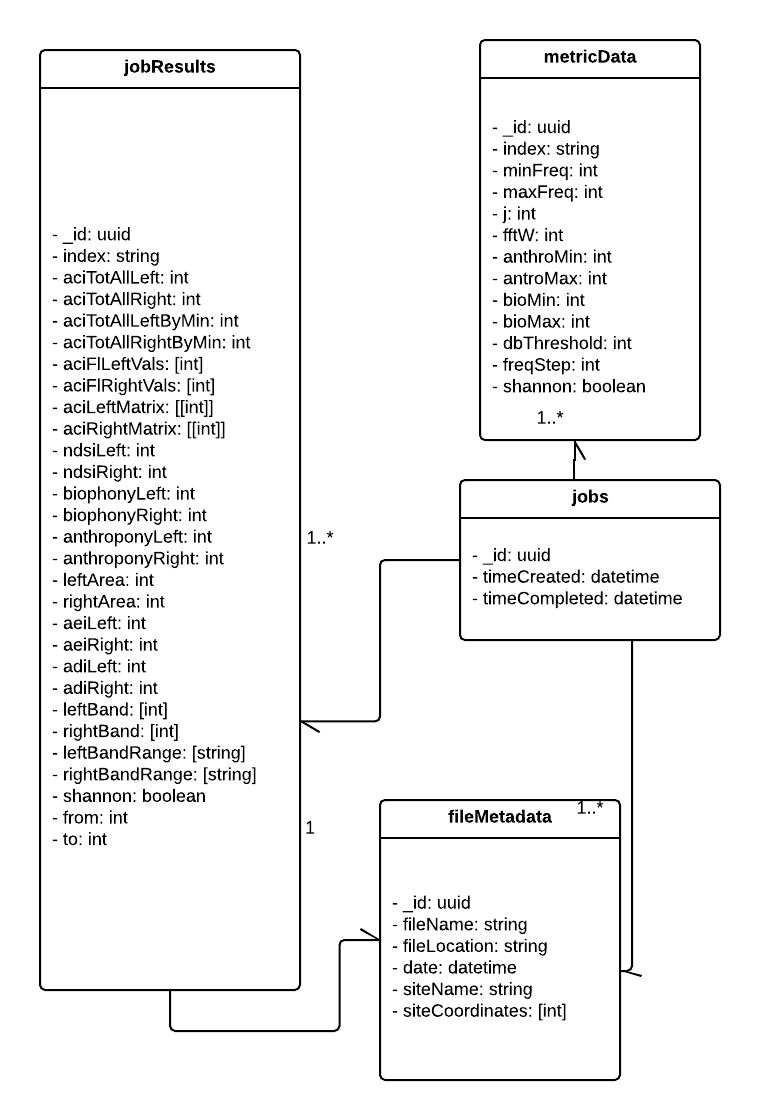
\includegraphics[width=.9\textwidth]{DBUML3}\\
As mentioned, jobs have a start and end time and date for use in creating graphs comparing results over time. In addition to these fields, jobs also have a reference to a fileMetadata object. The way that we have set up our database is that of an M to N relationship, where many jobs can be mapped to many different input sets.\par
The metric data collection represents the parameters used in each job. These parameters are index specific and job specific. We are deciding to keep track of these because it may be useful if the user wants to run the same job on a different data set, that way we are not storing redundant data.\par
These jobs produce outputs, as outlined in the job results collections. Each index has specific outputs based on what they are measuring. These output collections include references to the jobs and data sets that produced them.\par
\subsubsection{Overall Database}
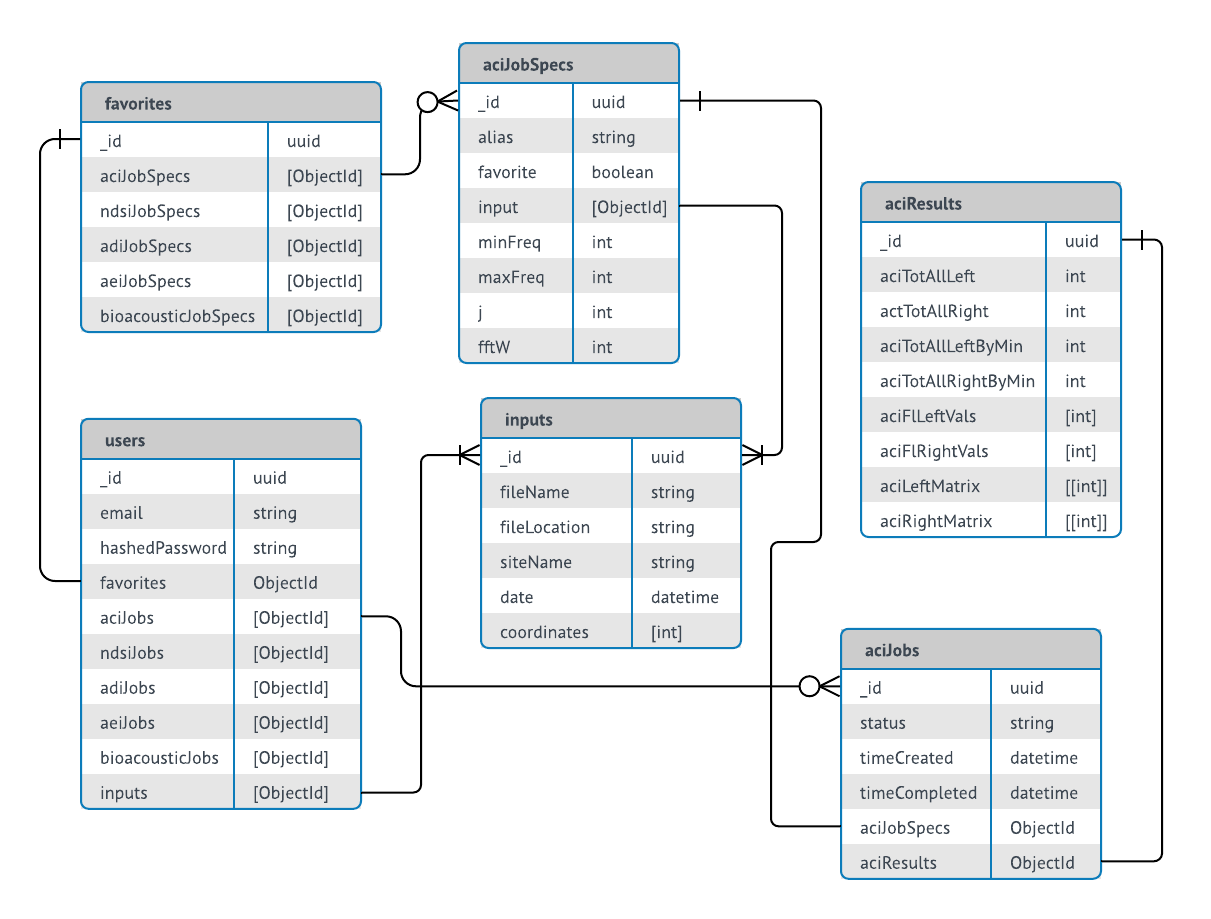
\includegraphics[width=\textwidth]{DBUML1}
Overall, this is the database implementation we will be using in our service. As outlined above, the pieces in the diagram will interact to produce an efficient and organized database to aid in user data storage and retrieval.\par
In this this visualization of the database, the ACI index is used as an example of how the collections realted to jobs will be referenced. Results and job specifications, or metric data for each other index will be represented in a similar way. This image shows the general structure of each collection for the other indices. \par
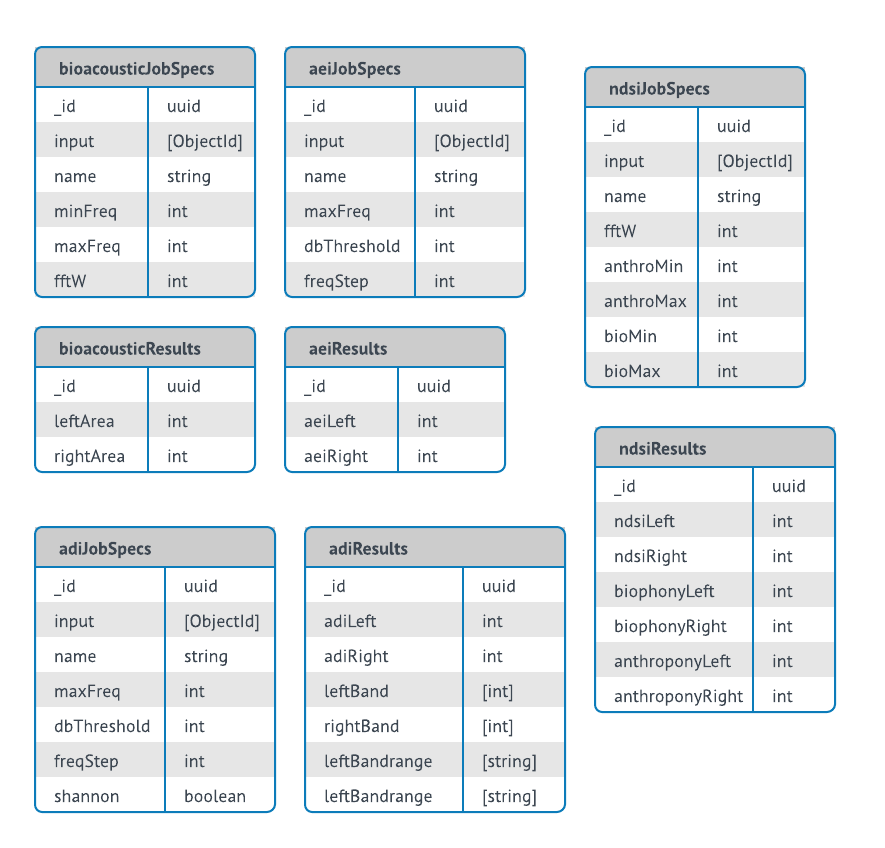
\includegraphics[width=\textwidth]{OtherCollections}